\documentclass[xcolor=svgnames,handout]{beamer}

\usepackage[utf8]    {inputenc}
\usepackage[T1]      {fontenc}
\usepackage[english] {babel}
\usepackage[super]{nth}
\usepackage{courier}
\usepackage{amsmath,amsfonts,graphicx}
\usepackage{beamerleanprogress}
\usepackage{comment}

\title{Semantic Frame Induction}
\subtitle {Course: Natural Language Processing I}

\author{Laura Aina, Eliška Hartlová, Francesco Stablum}


\institute[University of Amsterdam] % (optional, but mostly needed)

\date{November \nth{13} 2015}

\AtBeginSubsection[]
{
  \begin{frame}<beamer>{Outline}
    \tableofcontents[currentsection,currentsubsection]
  \end{frame}
}

\begin{document} 

\begin{frame}
  \titlepage
\end{frame}

\section{The task}

\begin{frame}{What is a semantic frame?}
  \begin{itemize}
  \item {
    A \textbf{semantic frame} is a schematization of the situation/event/state expressed by a predicative lexical item through the set of lexical items typically associated with it and their semantic roles.
    \begin {example}
    \textit{Mary eats an apple.} $\leadsto$ {Frame: Ingestion} \\ Mary \texttt{[NP-Subject-Ingestor]} eats \texttt{[VP-Predicate]} an apple \texttt{[NP-Direct Object - Ingestible ]}. 
    \end{example}
    \pause
  }
  \item {
    \textbf{Framenet} is a computational lexicon that contains frame-semantic descriptions of English lexical items, together with semantically annotated attestations in corpora.
  }
  \end{itemize}
\end{frame}

\begin{frame}{Framenet: an example}
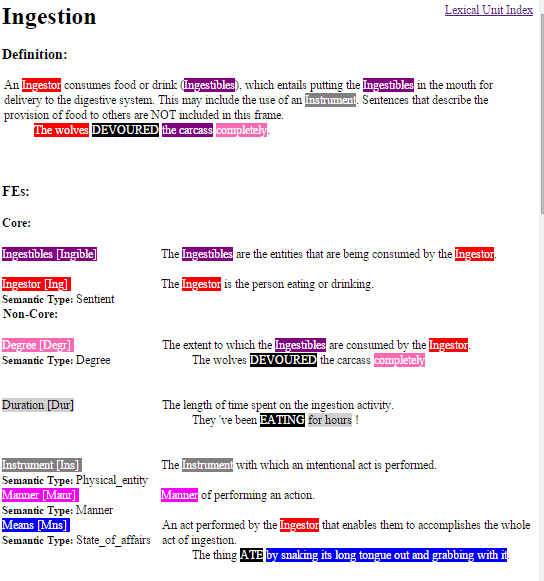
\includegraphics[width=55mm]{framenet1}
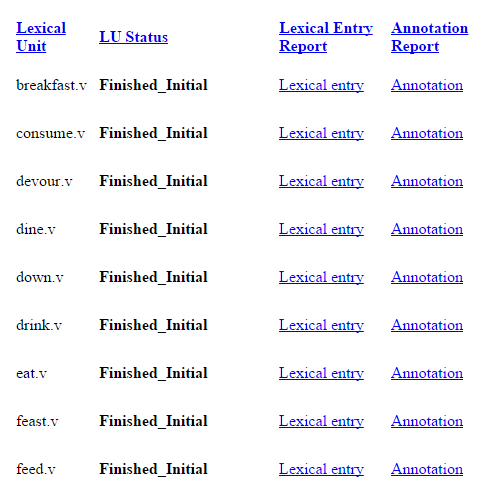
\includegraphics[width=55mm]{framenet2}
\end{frame}

\begin{frame}{Clustering verbs according to frames}
  \begin{itemize}
  \item {
    \textbf{Frame parsing} is the task of extracting frames from semantic predicate-argument structures.
    \pause 
  }
  \item {   
    In this case: clustering verbs according to frames given their arguments \textit{Subject} and \textit{Direct Object}.
  \begin{example}
    \textit{Mary eats an apple} $\leadsto$ \texttt{V: eat S: Mary DOBJ: apple}
  \end{example}
  }
  \end{itemize}
\end{frame}

\section{The data}
\begin{frame}{Building the dataset}
\begin{block}{Google Syntactic N-grams - English 1 Million Verbargs}
Set of n-grams (130M) consisting of verbs with all their immediate arguments
\begin{example}
\texttt {\tiny eats	while/IN/mark/3 he/PRP/nsubj/3 eats/VBZ/advcl/0 breakfast/NN/dobj/3	10	1950,2	1970,1	1976,1	1979,1	1993,2	1999,1	2001,1	2003,1}
\end{example}
\pause
\end{block}
\begin{block}{Preprocessing}
\begin{enumerate}
\item Extraction of triples: $V - S - DO$ \pause
\item Stemming \pause
\item Collapsing repetitions \pause
\item Filtering by the top n verbs/entries \pause
\end{enumerate}
\end{block}
\end{frame}

\section{Models}
\begin{frame}{Model 0}
	\begin{itemize}
		\item \textbf{Frame lexicon:} Dirichlet prior $\beta$. For each $f = 1..F$, sample three word multinomials: $\phi_f^{(v)}, \phi_f^{(s)}, \phi_f^{(o)} \sim  Dir(\beta)$
		%\vspace{0.5cm}
		\item \textbf{Tuple data:} For each tuple $i..N$,
		\begin{itemize}
			\item Draw its frame indicator $f_i$ (from a fixed prior)
			\item Draw the three words from their respective multinomials: $w_i^{(v)} \sim \phi_{f_i}^{(v)}; w_i^{(s)} \sim \phi_{f_i}^{(s)}; w_i^{(o)} \sim \phi_{f_i}^{(s)}$
		\end{itemize}
	\end{itemize}
	\begin{block}{Inference algorithm}
		EM
	\end{block}
	\begin{alertblock}{Assumption}
		Every tuple is modeled independently
	\end{alertblock}
\end{frame}
\begin{frame}{Model 1}
	\begin{itemize}
		\item F frames, and Dirichlet priors $\alpha, \beta$
		\item \textbf{Frame lexicon:} For each frame $f \in 1..F$, and argument position $a \in \{ 1,2,3\}$
		\begin{itemize}
			\item Draw word multinomial $\phi_f^{(a)} \sim Dir(\beta)$
		\end{itemize}
		\item \textbf{Document-tuple data:} For each document $d \in 1..D$
		\begin{itemize}
			\item Draw frame multinomial $\theta_d \sim Dir(\alpha)$
			\item For each tuple $i$ in the document,
			\begin{itemize}
				\item Draw frame indicator $f_i \sim \theta_d$
				\item Draw word triple: for each argument position $a \in \{ 1,2,3\}$\\
				%\begin{itemize}
				\hspace{0.5cm} Draw $w_i^{(a)} \sim \phi_{f_i}^{(a)}$
				%\end{itemize}
			\end{itemize}
		\end{itemize}
	\end{itemize}
	\begin{block}{Inference algorithm}
		Can be seen as LDA with ``frames'' instead of ``topics''
		\begin{itemize}
			\item Latent variable models syntactic arguments selection and document-level effects
			\item Collapsed Gibbs sampling
		\end{itemize}
	\end{block}
\end{frame}

\section{Evaluation}
\begin{frame}{Evaluation}
	\begin{itemize}
		\item Determine similarity between found clusters and those given by Framenet
		\item E.g. \textbf{Jaccard coefficient}: $Jacc(A,B) = \frac{|AB|}{A\cup B}$, where $A$ is the set of found items and $B$ the set of wanted items
	\end{itemize}
\end{frame}

\begin{comment}
\setbeamertemplate{bibliography item}[triangle]
\section{References}
\begin{frame}
    \nocite{*}
    \bibliographystyle{plain}
    \bibliography{bibliography}
\end{frame}
\end{comment}

\end{document}
